\subsection{Reputation Score}
\label{sec:reputation_score}

In order to construct the reputation of a transaction we construct a 4-tuple score (see Definition \ref{def:reputation_score}) based on the four transactional attributes of commit ranking (see Definition \ref{def:commit_ranking}), efficiency ranking (see Definition \ref{def:efficiency_ranking}), user ranking (see Definition \ref{def:user_ranking}), and system ranking (see Definition \ref{def:system_abort_ranking}). Each of the four values associated with the reputation score is a normalized value between 0 and 1 that ranks the transaction among all transactions executing within the system. Each value also contains a weighted multiplier that can be used in order to reward or place a higher precedence on a particular attribute for a particular transaction. If the multiplier is equal to one then all attributes contribute to the score equally.

Previously, the solution only kept commit rate and efficiency rate into consideration when categorizing transactions. This created a four category system that wouldn't allow dominance of transactions within the same category. By using the reputation score, we can now establish dominance of transactions that would originally have been in the same category. The next section discusses this dominance structure.

% In order to construct the reputation of a transaction class we use a bit-wise scoring system based on the four transactional attributes of commit ranking (see Definition \ref{def:commit_ranking}), efficiency ranking (see Definition \ref{def:efficiency_ranking}), user ranking (see Definition \ref{def:user_ranking}), and system ranking (see Definition \ref{def:system_abort_ranking}). The bit-wise score consists of using one byte for each attribute that can then be used to make more granular locking decisions. Our previous system of transactional categories (see Figure \ref{graph:cat_graph}) only allows for four possibilities of decision making. By moving to a bit-wise scoring system, we can then have a linear system of promoting and demoting transactions. This allows for a more granular approach that breaks down the walls of a strict four category system and allows for promotion and demotion of transactions that would normally be contained within the same category. With one byte representing each attribute (see Figure \ref{image:bitwise_reputation_score}), we then have 1,024 possible combinations that provide a much granular system than the previous four categories.

% The bit-wise score for each transaction will have one byte allocated for each transactional attribute for a total of thirty-two bits. From there we use positive reinforcement in order to increment or decrement the score. The scoring rules are shown below in Table \ref{tbl:scoring_matrix}.

% As you can see from the rules shown in Table \ref{tbl:scoring_matrix} we don't increment the individual scores unless they are within upper and lower twenty percentile. This prevents changing the score on every execution and allows the system to adjust gradually.


% \begin{table}[h]
% \captionsetup{justification=centering}
% \centering
% \begin{tabular}{|c|c|c|}
% \hline
% \multicolumn{2}{|c|}{\cellcolor[HTML]{EFEFEF}\textbf{Bit-Wise Scoring Values}}                                                   \\ \hline
% \textbf{Attribute Value} & \textbf{Scoring Value}   \\ \hline
% Commit Rate $<$ 20\%            &  -1        \\ \hline
% Commit Rate $>$ 80\%            &  +1        \\ \hline
% Efficiency Rate $<$ 20\%        &  +1        \\ \hline
% Efficiency Rate $>$ 80\%        &  -1        \\ \hline
% User Reputation $<$ 20\%        &  +1        \\ \hline
% User Reputation $>$ 80\%        &  -1        \\ \hline
% Forced Abort                    &  +2        \\ \hline
% Success after Forced Abort      &  -2        \\ \hline
% \end{tabular}

% \caption{Bit-Wise Scoring Matrix}
% \label{tbl:scoring_matrix} 

% \end{table}

% \begin{figure}
% \centering
% 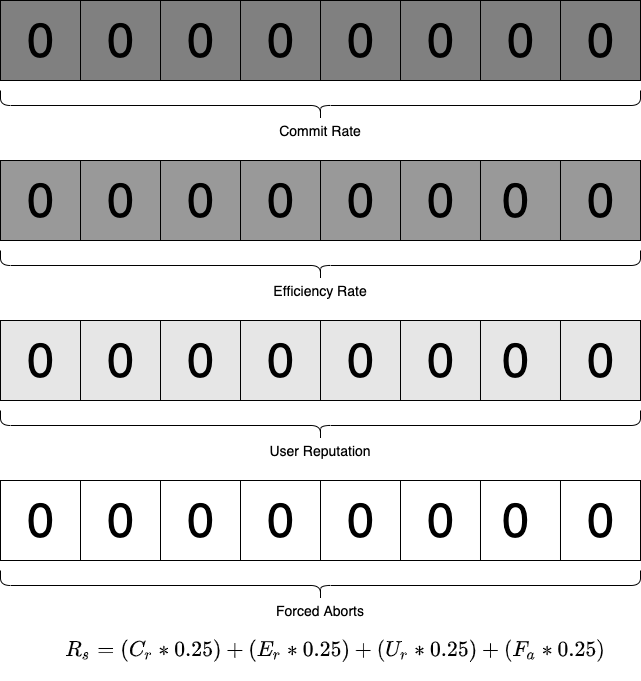
\includegraphics[scale=0.30]{images/BitwiseScore.png}
% \caption{Bit-Wise Reputation Score}
% \label{image:bitwise_reputation_score}
% \end{figure}